% ===========================================================================
% Spadafora Pierpaolo - Tesi di Laurea
% Euristiche di Dominio con Aggregati Dinamici in Answer Set Programming:
% Un Approccio Basato su Propagatori Nativi in Clingo
% ===========================================================================
\documentclass[a4paper,12pt,twoside,openright]{report}

% ---- Codifica e lingua ----
\usepackage[utf8]{inputenc}
\usepackage[T1]{fontenc}
\usepackage[italian]{babel}

% ---- Geometria ----
\usepackage[top=3cm,bottom=3cm,left=3.5cm,right=2.5cm]{geometry}

% ---- Tipografia ----
\usepackage{lmodern}
\usepackage{microtype}
\usepackage{setspace}
\onehalfspacing

% ---- Matematica ----
\usepackage{amsmath,amssymb,amsthm}

% ---- Algoritmi e codice ----
\usepackage{algorithm}
\usepackage{algpseudocode}
\usepackage{listings}
\usepackage{xcolor}

% ---- Grafici e figure ----
\usepackage{graphicx}
\usepackage{subcaption}
\usepackage{float}
\usepackage{booktabs}

% ---- Riferimenti ----
\usepackage{hyperref}
\hypersetup{
    colorlinks=true,
    linkcolor=blue!60!black,
    citecolor=green!50!black,
    urlcolor=blue!70!black,
}

% ---- Bibliografia ----
\usepackage[numbers,sort&compress]{natbib}

% ---- Teoremi ----
\newtheorem{definition}{Definizione}[chapter]
\newtheorem{theorem}{Teorema}[chapter]
\newtheorem{proposition}{Proposizione}[chapter]
\newtheorem{example}{Esempio}[chapter]

% ---- Listings per ASP e C++ ----
\definecolor{codegreen}{rgb}{0,0.6,0}
\definecolor{codegray}{rgb}{0.5,0.5,0.5}
\definecolor{codepurple}{rgb}{0.58,0,0.82}
\definecolor{backcolour}{rgb}{0.97,0.97,0.97}

\lstdefinestyle{aspstyle}{
    backgroundcolor=\color{backcolour},
    commentstyle=\color{codegreen},
    keywordstyle=\color{blue},
    numberstyle=\tiny\color{codegray},
    stringstyle=\color{codepurple},
    basicstyle=\ttfamily\footnotesize,
    breakatwhitespace=false,
    breaklines=true,
    captionpos=b,
    keepspaces=true,
    numbers=left,
    numbersep=5pt,
    showspaces=false,
    showstringspaces=false,
    showtabs=false,
    tabsize=2,
    frame=single,
    rulecolor=\color{codegray},
}

\lstdefinestyle{cppstyle}{
    backgroundcolor=\color{backcolour},
    commentstyle=\color{codegreen},
    keywordstyle=\color{blue},
    numberstyle=\tiny\color{codegray},
    stringstyle=\color{codepurple},
    basicstyle=\ttfamily\footnotesize,
    breakatwhitespace=false,
    breaklines=true,
    captionpos=b,
    keepspaces=true,
    numbers=left,
    numbersep=5pt,
    showspaces=false,
    showstringspaces=false,
    showtabs=false,
    tabsize=2,
    frame=single,
    rulecolor=\color{codegray},
    language=C++,
    morekeywords={override,noexcept,nullptr,auto,final,unique_ptr},
}

\lstset{style=aspstyle}

% ---- Comandi personalizzati ----
\newcommand{\clingo}{\texttt{clingo}}
\newcommand{\wasp}{\texttt{WASP}}
\newcommand{\alphasys}{\textsc{Alpha}}
\newcommand{\asp}{\textsc{ASP}}
\newcommand{\cdcl}{\textsc{CDCL}}
\newcommand{\vsids}{\textsc{VSIDS}}
\newcommand{\hprop}{\texttt{HeuristicPropagator}}

% ===========================================================================
\begin{document}

% ---- Frontespizio ----
\begin{titlepage}
    \centering
    \vspace*{1cm}

    {\Large \textsc{Universit\`{a} della Calabria}}\\[0.3cm]
    {\large Dipartimento di Matematica e Informatica}\\[0.3cm]
    {\large Corso di Laurea in Informatica}\\[2cm]

    {\Huge \textbf{Euristiche di Dominio con\\Aggregati Dinamici in\\Answer Set Programming}}\\[0.5cm]
    {\Large Un Approccio Basato su Propagatori Nativi in Clingo}\\[3cm]

    \begin{minipage}[t]{0.45\textwidth}
        \raggedright
        {\large \textbf{Relatore:}}\\[0.2cm]
        {\large Prof. Francesco Calimeri}\\[0.5cm]
        {\large \textbf{Correlatore:}}\\[0.2cm]
        {\large Dott. Javier Romero}
    \end{minipage}
    \hfill
    \begin{minipage}[t]{0.45\textwidth}
        \raggedleft
        {\large \textbf{Candidato:}}\\[0.2cm]
        {\large Pierpaolo Spadafora}\\[0.2cm]
    \end{minipage}

    \vfill
    {\large Anno Accademico 2024/2025}
\end{titlepage}

% ---- Indice ----
\tableofcontents
\newpage

% ===========================================================================
% CAPITOLO 1: INTRODUZIONE
% ===========================================================================
\chapter{Introduzione}
\label{ch:introduzione}

\section{Il Paradigma dell'Answer Set Programming}

L'\emph{Answer Set Programming} (ASP) \`{e} un paradigma di programmazione dichiarativa orientato alla risoluzione di problemi combinatori complessi. In ASP, un problema viene codificato come un programma logico il cui significato \`{e} dato dalla semantica degli \emph{answer set} (o \emph{modelli stabili}), introdotta da Gelfond e Lifschitz nel 1988. Ogni answer set rappresenta una soluzione al problema codificato.

Il ciclo di vita di un programma ASP si articola in due fasi principali:
\begin{enumerate}
    \item \textbf{Grounding}: il programma con variabili viene istanziato (``\emph{grounded}''), producendo un programma proposizionale equivalente. Questa fase \`{e} svolta da un componente detto \emph{grounder} (ad esempio \texttt{gringo} nel sistema \clingo{}).
    \item \textbf{Solving}: il programma ground viene passato a un risolutore SAT/ASP (il \emph{solver}), che calcola gli answer set utilizzando algoritmi derivati da \cdcl{} (\emph{Conflict-Driven Clause Learning}).
\end{enumerate}

\section{Il Problema del Grounding Bottleneck}
\label{sec:grounding_bottleneck}

Il \emph{grounding bottleneck} rappresenta una delle principali limitazioni nell'applicazione pratica dell'ASP a domini reali. Durante la fase di grounding, regole contenenti variabili e, in particolare, aggregati vengono espanse in tutte le possibili istanziazioni. Quando il dominio \`{e} grande o quando compaiono aggregati nelle condizioni delle euristiche di dominio, il numero di regole ground pu\`{o} crescere esponenzialmente.

Si consideri ad esempio la seguente direttiva euristica per il \emph{Balanced Sum Problem} (BSP):
\begin{lstlisting}[caption={Euristica di dominio con aggregato nella condizione}]
#heuristic b(X) : x(X), not c(X), S = #sum{Y : c(Y)}. [X@S, true]
\end{lstlisting}

Per un dominio di dimensione $n$, il grounder deve produrre una regola ground per \emph{ogni possibile valore} dell'aggregato $S = \#sum\{Y : c(Y)\}$. Il numero di tali regole \`{e} $\mathcal{O}(n \cdot 2^n)$, poich\'{e} la somma pu\`{o} assumere fino a $\sum_{i=1}^{n} i = n(n+1)/2$ valori distinti.

\begin{example}
Per $n=3$, il grounding della prima euristica produce le seguenti 7 regole per ciascun valore di $X$:
\begin{lstlisting}
#heuristic b(1):not c(1),#sum{1:c(1);2:c(2);3:c(3)}=0.[1@0,true]
#heuristic b(1):not c(1),#sum{1:c(1);2:c(2);3:c(3)}=1.[1@1,true]
...
#heuristic b(1):not c(1),#sum{1:c(1);2:c(2);3:c(3)}=6.[1@6,true]
\end{lstlisting}
Per tutte le variabili e per entrambe le euristiche, il numero totale di regole ground \`{e} $2 \times n \times (n(n+1)/2 + 1) = \mathcal{O}(n^3)$ nel caso del BSP.
\end{example}

\section{Obiettivo della Tesi}

L'obiettivo di questa tesi \`{e} dimostrare la fattibilit\`{a} di un approccio che aggira il grounding bottleneck per le euristiche di dominio contenenti aggregati dinamici. L'idea chiave consiste nel:
\begin{enumerate}
    \item Riscrivere le direttive \texttt{\#heuristic} standard come regole ordinarie con un predicato speciale \texttt{\_\_heuristic/4}, codificando l'aggregato come funzione non interpretata (ad esempio \texttt{\_\_sum(c)}).
    \item Implementare un \emph{propagatore nativo} nel codice C++ di \clingo{} che intercetta le direttive riscritte, calcola gli aggregati dinamicamente durante la ricerca, e guida la scelta dei letterali nel \emph{decision loop}.
\end{enumerate}

Il lavoro si articola in tre fasi, come descritto nel documento di specifica del progetto:
\begin{enumerate}
    \item \textbf{Studio preliminare}: comprensione dell'approccio alle euristiche con lazy grounding.
    \item \textbf{Implementazione del caso base}: propagatore per euristiche con atomi ground e singolo letterale nel corpo.
    \item \textbf{Estensione al caso non-ground}: valutazione dinamica degli aggregati nel propagatore, con grounding on-demand della priorit\`{a}.
\end{enumerate}

\section{Struttura del Documento}

La tesi \`{e} organizzata come segue:
\begin{itemize}
    \item Il \textbf{Capitolo~\ref{ch:stato_arte}} presenta lo stato dell'arte sul lazy grounding e sulle euristiche di dominio nei solutori ASP.
    \item Il \textbf{Capitolo~\ref{ch:architettura}} descrive l'architettura dell'implementazione, con particolare attenzione all'integrazione nel ciclo di propagazione di \clingo{}.
    \item Il \textbf{Capitolo~\ref{ch:aggregati}} dettaglia la progettazione degli stati aggregati dinamici e la loro complessit\`{a} computazionale.
    \item Il \textbf{Capitolo~\ref{ch:sperimentale}} presenta e discute i risultati sperimentali sul Balanced Sum Problem.
    \item Il \textbf{Capitolo~\ref{ch:conclusioni}} conclude con un riepilogo dei contributi e una discussione delle limitazioni e degli sviluppi futuri.
\end{itemize}

% ===========================================================================
% CAPITOLO 2: STATO DELL'ARTE
% ===========================================================================
\chapter{Stato dell'Arte}
\label{ch:stato_arte}

\section{Fondamenti di ASP}

Un \emph{programma logico} in ASP \`{e} un insieme finito di regole della forma:
\begin{equation}
    a_1 \vee \cdots \vee a_k \leftarrow b_1, \ldots, b_m, \mathit{not}\; c_1, \ldots, \mathit{not}\; c_n
\end{equation}
dove $a_i$, $b_j$, $c_l$ sono atomi proposizionali. La parte sinistra della regola \`{e} detta \emph{testa}, la parte destra \`{e} il \emph{corpo}. Le regole con testa vuota sono \emph{vincoli di integrit\`{a}}.

\begin{definition}[Answer Set]
Dato un programma logico $P$, un insieme $I$ di atomi \`{e} un \emph{answer set} di $P$ se $I$ \`{e} un modello minimale del \emph{ridotto di Gelfond-Lifschitz} $P^I$.
\end{definition}

\section{Il Ciclo Grounding-Solving}

I sistemi ASP moderni, come \clingo{} e \wasp{}, adottano un'architettura a due fasi:
\begin{enumerate}
    \item Il \emph{grounder} (\texttt{gringo} in \clingo{}) trasforma il programma con variabili in un programma proposizionale ground.
    \item Il \emph{solver} (\texttt{clasp} in \clingo{}) ricerca gli answer set del programma ground tramite algoritmi \cdcl{}.
\end{enumerate}

L'algoritmo \cdcl{} \`{e} un'estensione del \emph{DPLL} che include \emph{clause learning} e \emph{non-chronological backtracking}. Ad ogni passo di decisione, il solver sceglie un letterale non assegnato secondo un'\emph{euristica di branching} e ne propaga le conseguenze logiche. In caso di conflitto, viene appresa una nuova clausola e l'algoritmo effettua backtracking.

\section{Euristiche di Branching: da VSIDS alle Euristiche di Dominio}
\label{sec:vsids}

L'euristica di branching determina quale letterale assegnare ad ogni punto di decisione. La scelta dell'euristica ha un impatto significativo sulle prestazioni del solver.

\subsection{VSIDS}

La \emph{Variable State Independent Decaying Sum} (\vsids{}) \`{e} l'euristica di branching pi\`{u} utilizzata nei solver SAT moderni. Introdotta da Chaff, \vsids{} mantiene un contatore di attivit\`{a} per ciascuna variabile, incrementato ogni volta che la variabile compare in una clausola appresa. I contatori vengono periodicamente scalati (``\emph{decayed}'') di un fattore costante, privilegiando cos\`{i} le variabili coinvolte nei conflitti pi\`{u} recenti.

\vsids{} \`{e} un'euristica \emph{domain-independent}: non utilizza alcuna conoscenza del dominio del problema. Sebbene sia estremamente efficace per problemi SAT generici, pu\`{o} essere subottimale per problemi combinatori strutturati dove esiste conoscenza specifica del dominio.

\subsection{Euristiche di Dominio in ASP}

Le \emph{euristiche di dominio} (domain-specific heuristics) permettono all'utente di guidare la ricerca del solver codificando conoscenza euristica direttamente nel programma ASP. In \clingo{}, la direttiva:
\begin{lstlisting}[caption={Sintassi della direttiva euristica in Clingo}]
#heuristic atom : body. [weight@priority, sign]
\end{lstlisting}
specifica che, quando il corpo \texttt{body} \`{e} soddisfatto, l'atomo \texttt{atom} dovrebbe essere scelto con il peso \texttt{weight} al livello di priorit\`{a} \texttt{priority} e con il segno \texttt{sign} (\texttt{true} o \texttt{false}).

L'algoritmo di selezione opera come segue:
\begin{enumerate}
    \item Si selezionano tutte le direttive euristiche la cui condizione \`{e} soddisfatta nell'assegnamento parziale corrente.
    \item Tra queste, si sceglie il target con il \emph{livello di priorit\`{a}} massimo.
    \item A parit\`{a} di livello, si sceglie il target con il \emph{peso} massimo.
    \item Se nessuna direttiva \`{e} applicabile (o il target \`{e} gi\`{a} assegnato), il solver ripristina la sua euristica di default (\vsids{}).
\end{enumerate}

Dodaro et al.\ hanno dimostrato l'efficacia delle euristiche di dominio su diversi benchmark combinatori, inclusi problemi di scheduling e configurazione.

\section{Il Lazy Grounding}
\label{sec:lazy_grounding}

Il lazy grounding \`{e} un approccio alternativo al grounding tradizionale in cui le regole vengono istanziate \emph{incrementalmente} durante la ricerca, piuttosto che completamente prima di essa. L'obiettivo \`{e} evitare l'esplosione combinatoria prodotta dal grounding completo.

Nel contesto delle euristiche di dominio, il lazy grounding assume un significato particolare: anzich\'{e} istanziare esplicitamente ogni possibile combinazione di aggregato e variabili, si calcola il valore dell'aggregato \emph{dinamicamente} durante la ricerca, basandosi sull'assegnamento parziale corrente.

\subsection{Il Sistema Alpha}

Il sistema Alpha, sviluppato da Weinzierl et al., adotta un approccio completamente lazy al grounding, basato su Prolog. L'architettura di Alpha prevede che il grounder sia integrato con il solver in un ciclo unico: le regole vengono istanziate solamente quando diventano applicabili, e le euristiche vengono valutate dinamicamente tramite query Datalog al grounder.

Nell'approccio di Alpha:
\begin{itemize}
    \item Le euristiche di dominio sono valutate tramite un meccanismo di \emph{query-driven evaluation} che interroga il grounder durante la fase di decisione.
    \item Il valore dell'aggregato \`{e} calcolato effettuando una query sull'insieme dei fatti derivati fino a quel punto della ricerca.
    \item L'approccio \`{e} concettualmente pulito ma introduce overhead significativo, poich\'{e} il grounder \`{e} implementato in Prolog/Java e ogni query implica il traversamento dell'intero stato corrente.
\end{itemize}

\subsection{Aggregati Dinamici nelle Euristiche}
\label{sec:aggregati_dinamici_letteratura}

Romero et al.\ hanno introdotto il concetto di \emph{aggregati dinamici} nelle euristiche di dominio per risolvere problemi di configurazione come il \emph{Partner Units Problem} (PUP). In questo contesto, la priorit\`{a} dell'euristica dipende da funzioni aggregate (somma, conteggio, minimo, massimo) calcolate sull'assegnamento parziale corrente.

L'aspetto critico \`{e} che il grounding tradizionale di tali euristiche produce un numero esponenziale di regole ground, rendendo il solver inutilizzabile per istanze di dimensione realistica. L'approccio proposto prevede di valutare gli aggregati \emph{a runtime} durante la ricerca, mantenendo strutture dati incrementali che supportino le operazioni di aggiunta, rimozione e interrogazione in tempo costante o logaritmico.

% ===========================================================================
% CAPITOLO 3: ARCHITETTURA DELL'IMPLEMENTAZIONE
% ===========================================================================
\chapter{Architettura dell'Implementazione}
\label{ch:architettura}

\section{Scelta dell'Approccio}

A differenza dell'approccio query-driven adottato dal sistema Alpha (basato su Prolog), la nostra implementazione opera come un \emph{propagatore nativo} scritto in C++ e integrato direttamente nel ciclo di ricerca di \clingo{}. Questa scelta offre diversi vantaggi:

\begin{enumerate}
    \item \textbf{Prestazioni}: essendo compilato in C++ e integrato nel solutore, il propagatore evita il costo delle chiamate inter-processo e della serializzazione dei dati.
    \item \textbf{Accesso diretto al trail}: il propagatore ha accesso diretto all'assegnamento parziale (\texttt{Assignment}) e al trail del solver, permettendo aggiornamenti in tempo $\mathcal{O}(1)$ per operazione.
    \item \textbf{Backtracking nativo}: il meccanismo di \texttt{undo} del propagatore \`{e} invocato automaticamente dal solver durante il backtracking, garantendo la correttezza dello stato senza overhead aggiuntivo.
\end{enumerate}

\section{L'Interfaccia Heuristic di Clingo}
\label{sec:interfaccia_heuristic}

\clingo{} espone l'interfaccia \texttt{Clingo::Heuristic}, che estende \texttt{Clingo::Propagator} con il metodo \texttt{decide}:

\begin{lstlisting}[style=cppstyle,caption={Interfaccia \texttt{Heuristic} di Clingo}]
class Heuristic : public Propagator {
    // Ereditati da Propagator:
    virtual void init(PropagateInit &init);
    virtual void propagate(PropagateControl &ctl, LiteralSpan changes);
    virtual void undo(PropagateControl const &ctl, LiteralSpan changes) noexcept;

    // Specifico di Heuristic:
    virtual literal_t decide(id_t thread_id, Assignment const &assignment,
                             literal_t fallback);
};
\end{lstlisting}

Il metodo \texttt{decide} viene invocato dal solver ad ogni punto di decisione. Se restituisce un letterale diverso da $0$, il solver lo adotta come decisione corrente; se restituisce $0$, il solver ricade sulla sua euristica di default (\vsids{}).

\section{Riscrittura delle Direttive Euristiche}
\label{sec:riscrittura}

La chiave dell'approccio consiste nella riscrittura delle direttive \texttt{\#heuristic} standard in regole ordinarie con il predicato speciale \texttt{\_\_heuristic/4}:

\begin{lstlisting}[caption={Trasformazione della direttiva euristica}]
% Originale:
#heuristic b(X) : x(X), not c(X), S = #sum{Y : c(Y)}. [X@S, true]

% Riscritta:
__heuristic(b(X), X, __sum(c), true) :- x(X), not c(X).
\end{lstlisting}

Nella forma riscritta:
\begin{itemize}
    \item Il primo argomento (\texttt{b(X)}) \`{e} il \emph{target}: l'atomo che l'euristica suggerisce di rendere vero o falso.
    \item Il secondo argomento (\texttt{X}) \`{e} il \emph{peso} statico.
    \item Il terzo argomento (\texttt{\_\_sum(c)}) \`{e} la \emph{priorit\`{a} dinamica}: una funzione non interpretata che il propagatore valuter\`{a} a runtime calcolando la somma dei valori degli atomi \texttt{c/1} attualmente veri.
    \item Il quarto argomento (\texttt{true}) \`{e} il \emph{segno} della decisione.
\end{itemize}

L'aggregato, codificato come termine funzionale \texttt{\_\_sum(c)}, non viene valutato dal grounder: essendo un simbolo funzionale privo di semantica nel linguaggio, il grounder lo tratta come un valore costante. Il grounder di \clingo{} istanzia la regola per ogni valore di \texttt{X} presente nel dominio, ma senza espandere i possibili valori della somma. Il risultato \`{e} un numero di regole ground \emph{lineare} in $n$, anzich\'{e} esponenziale.

\section{Ciclo di Vita del Propagatore}
\label{sec:ciclo_vita}

Il propagatore \hprop{} partecipa al ciclo di ricerca di \clingo{} attraverso quattro callback:

\begin{enumerate}
    \item \texttt{init}: invocata una volta prima della ricerca. Il propagatore:
    \begin{itemize}
        \item Scansiona gli atomi simbolici alla ricerca di \texttt{\_\_heuristic/4}.
        \item Per ciascun atomo trovato, estrae target, peso, chiave aggregata e il letterale dell'atomo \texttt{\_\_heuristic} stesso.
        \item Registra i \emph{watch} sui letterali dei predicati da aggregare.
    \end{itemize}

    \item \texttt{propagate}: invocata quando un letterale osservato diventa vero. Il propagatore aggiorna lo stato dell'aggregato corrispondente con l'operazione \texttt{add}.

    \item \texttt{undo}: invocata durante il backtracking. Il propagatore annulla l'aggiornamento con l'operazione \texttt{remove}.

    \item \texttt{decide}: invocata ad ogni punto di decisione. Il propagatore:
    \begin{itemize}
        \item Verifica che la condizione dell'euristica sia soddisfatta (l'atomo \texttt{\_\_heuristic} deve essere vero).
        \item Verifica che il target sia ancora libero (non assegnato).
        \item Legge il valore corrente dell'aggregato in $\mathcal{O}(1)$.
        \item Seleziona il target con priorit\`{a} massima; a parit\`{a}, con peso massimo.
        \item Restituisce $0$ se nessun target \`{e} applicabile (fallback a \vsids{}).
    \end{itemize}
\end{enumerate}

\begin{figure}[H]
    \centering
    \fbox{%
    \begin{minipage}{0.85\textwidth}
    \begin{algorithmic}[1]
        \Function{decide}{$\mathit{assignment}$}
            \State $\mathit{best} \gets 0$
            \State $\mathit{max\_prio} \gets -1$, $\mathit{best\_weight} \gets -1$
            \ForAll{$t \in \mathit{heuristic\_targets}$}
                \If{$\mathit{assignment}[t.\mathit{heuristic\_lit}] \neq \textsc{True}$}
                    \State \textbf{continue} \Comment{Condizione non soddisfatta}
                \EndIf
                \If{$\mathit{assignment}[t.\mathit{lit}] \neq \textsc{Free}$}
                    \State \textbf{continue} \Comment{Target gi\`{a} assegnato}
                \EndIf
                \State $p \gets \mathit{aggregate\_states}[t.\mathit{agg\_key}].\mathit{result}()$
                \If{$p > \mathit{max\_prio}$ \textbf{or} ($p = \mathit{max\_prio}$ \textbf{and} $t.\mathit{weight} > \mathit{best\_weight}$)}
                    \State $\mathit{max\_prio} \gets p$, $\mathit{best\_weight} \gets t.\mathit{weight}$
                    \State $\mathit{best} \gets t.\mathit{lit}$
                \EndIf
            \EndFor
            \State \Return $\mathit{best}$
        \EndFunction
    \end{algorithmic}
    \end{minipage}
    }
    \caption{Pseudocodice dell'algoritmo di decisione del \hprop{}}
    \label{fig:decide_algorithm}
\end{figure}

\section{Verifica della Condizione dell'Euristica}
\label{sec:verifica_condizione}

Un aspetto critico dell'implementazione \`{e} la verifica che la \emph{condizione} dell'euristica sia effettivamente soddisfatta prima di applicarla. Poich\'{e} le direttive euristiche sono riscritte come regole ordinarie (\texttt{\_\_heuristic(...) :- body}), \`{e} il solver standard di \clingo{} a valutare il corpo della regola. Quando il corpo \`{e} soddisfatto, l'atomo \texttt{\_\_heuristic(...)} diventa vero nel trail.

Durante la fase di inizializzazione (\texttt{init}), il propagatore memorizza il \texttt{solver\_literal} dell'atomo \texttt{\_\_heuristic} stesso (non solo del target). Nel metodo \texttt{decide}, prima di considerare un target, il propagatore verifica che il corrispondente atomo \texttt{\_\_heuristic} sia valutato a \texttt{True} nell'assegnamento corrente:

\begin{lstlisting}[style=cppstyle,caption={Verifica della condizione nel metodo \texttt{decide}}]
for (auto const &target_info : heuristic_targets_) {
    // L'atomo __heuristic(...) deve essere True
    if (assignment.truth_value(target_info.heuristic_lit)
        != Clingo::TruthValue::True) {
        continue;
    }
    // Il target deve essere Free
    if (assignment.truth_value(target_info.lit)
        != Clingo::TruthValue::Free) {
        continue;
    }
    // ... selezione basata su priority e weight
}
\end{lstlisting}

Senza questo controllo, il propagatore applicherebbe ciecamente le priorit\`{a} a target le cui condizioni logiche potrebbero essere false o non ancora derivate, violando la semantica delle direttive euristiche.

\section{Confronto con l'Approccio di Alpha}

\begin{table}[H]
    \centering
    \caption{Confronto tra l'approccio nativo (Clingo) e l'approccio query-driven (Alpha)}
    \label{tab:confronto_alpha}
    \begin{tabular}{lcc}
        \toprule
        \textbf{Caratteristica} & \textbf{Propagatore Nativo} & \textbf{Alpha (Query-Driven)} \\
        \midrule
        Linguaggio               & C++ (nativo)        & Prolog/Java \\
        Integrazione             & Interno al solver   & Chiamata esterna \\
        Aggiornamento aggregato  & $\mathcal{O}(1)$ incrementale   & $\mathcal{O}(n)$ query completa \\
        Backtracking             & Automatico (undo)   & Ricostruzione stato \\
        Overhead per decisione   & Costante            & Lineare nel dominio \\
        Supporto aggregati       & Sum, Count, Min, Max & Tutti (via Prolog) \\
        Estensibilit\`{a}        & Richiede nuovo codice C++ & Regole Prolog \\
        \bottomrule
    \end{tabular}
\end{table}

% ===========================================================================
% CAPITOLO 4: AGGREGATI DINAMICI
% ===========================================================================
\chapter{Progettazione degli Stati Aggregati Dinamici}
\label{ch:aggregati}

\section{L'Interfaccia AggregateState}

Per supportare diversi tipi di aggregati in maniera uniforme, abbiamo adottato un design basato sul \emph{polimorfismo a runtime} tramite una classe base astratta \texttt{AggregateState}:

\begin{lstlisting}[style=cppstyle,caption={Interfaccia \texttt{AggregateState}}]
struct AggregateState {
    virtual ~AggregateState() = default;

    virtual void add(int value) = 0;    // Atomo diventa vero
    virtual void remove(int value) = 0; // Backtracking
    virtual int result() const = 0;     // Valore corrente
    virtual void reset() = 0;           // Ripristino iniziale
};
\end{lstlisting}

Il propagatore non conosce mai il tipo concreto dell'aggregato: utilizza esclusivamente l'interfaccia base. Questo consente di estendere il sistema con nuovi aggregati senza modificare la logica del propagatore.

\section{Implementazioni Concrete}

\subsection{SumState (\_\_sum)}

Lo stato per l'aggregato somma mantiene un accumulatore intero:

\begin{lstlisting}[style=cppstyle,caption={Implementazione di \texttt{SumState}}]
struct SumState final : AggregateState {
    int total = 0;
    void add(int v) override    { total += v; }
    void remove(int v) override { total -= v; }
    int result() const override { return total; }
    void reset() override       { total = 0; }
};
\end{lstlisting}

\begin{proposition}[Complessit\`{a} di SumState]
Tutte le operazioni (\texttt{add}, \texttt{remove}, \texttt{result}) hanno complessit\`{a} temporale $\mathcal{O}(1)$ e complessit\`{a} spaziale $\mathcal{O}(1)$.
\end{proposition}

\subsection{CountState (\_\_count)}

Lo stato per il conteggio \`{e} analogo a \texttt{SumState}, ma ignora il valore numerico dell'atomo:

\begin{lstlisting}[style=cppstyle,caption={Implementazione di \texttt{CountState}}]
struct CountState final : AggregateState {
    int count = 0;
    void add(int) override      { ++count; }
    void remove(int) override   { --count; }
    int result() const override { return count; }
    void reset() override       { count = 0; }
};
\end{lstlisting}

\begin{proposition}[Complessit\`{a} di CountState]
Tutte le operazioni hanno complessit\`{a} $\mathcal{O}(1)$ in tempo e $\mathcal{O}(1)$ in spazio.
\end{proposition}

\subsection{MinState e MaxState (\_\_min, \_\_max)}

Per gli aggregati di minimo e massimo, non \`{e} sufficiente un singolo accumulatore, poich\'{e} la rimozione di un valore potrebbe alterare il risultato. Adottiamo una \texttt{std::map<int,int>} (albero bilanciato) che mappa ciascun valore al suo conteggio di occorrenze:

\begin{lstlisting}[style=cppstyle,caption={Implementazione di \texttt{MinState}}]
struct MinState final : AggregateState {
    std::map<int, int> active; // valore -> conteggio
    void add(int v) override    { active[v]++; }
    void remove(int v) override {
        auto it = active.find(v);
        if (it != active.end()) {
            if (--(it->second) == 0) active.erase(it);
        }
    }
    int result() const override {
        return active.empty() ? INT_MAX : active.begin()->first;
    }
    void reset() override { active.clear(); }
};
\end{lstlisting}

\begin{proposition}[Complessit\`{a} di MinState/MaxState]
Le operazioni \texttt{add} e \texttt{remove} hanno complessit\`{a} $\mathcal{O}(\log k)$, dove $k$ \`{e} il numero di valori distinti attivi. L'operazione \texttt{result} ha complessit\`{a} $\mathcal{O}(1)$ (accesso al primo/ultimo elemento di una mappa ordinata). La complessit\`{a} spaziale \`{e} $\mathcal{O}(k)$.
\end{proposition}

\section{Chiave Aggregata Composita}

Ogni aggregato \`{e} identificato univocamente da una \texttt{AggregateKey} composta da tre campi:

\begin{lstlisting}[style=cppstyle,caption={Struttura \texttt{AggregateKey}}]
struct AggregateKey {
    std::string op;     // Es: "__sum"
    std::string pred;   // Es: "c"
    int arg_index = -1; // Indice dell'argomento numerico (-1 = ultimo)

    bool operator==(AggregateKey const &o) const {
        return op == o.op && pred == o.pred && arg_index == o.arg_index;
    }
};
\end{lstlisting}

Il campo \texttt{arg\_index} consente di specificare quale argomento di un predicato n-ario contiene il valore numerico da aggregare. Ad esempio, per il predicato \texttt{assigned\_zone\_unit(Z, U)} del Partner Units Problem, si userebbe \texttt{\_\_sum(assigned\_zone\_unit, 1)} per aggregare sul secondo argomento.

La factory function \texttt{make\_aggregate} crea l'implementazione concreta appropriata:

\begin{lstlisting}[style=cppstyle,caption={Factory function per gli aggregati}]
std::unique_ptr<AggregateState> make_aggregate(std::string const &op_name) {
    if (op_name == "__sum")   return std::make_unique<SumState>();
    if (op_name == "__count") return std::make_unique<CountState>();
    if (op_name == "__min")   return std::make_unique<MinState>();
    if (op_name == "__max")   return std::make_unique<MaxState>();
    return nullptr;
}
\end{lstlisting}

\section{Supporto per Predicati N-ari}

Una limitazione iniziale del propagatore era il supporto esclusivo per predicati di arità 1. Per supportare predicati con arità arbitraria, la seconda passata della fase di inizializzazione utilizza l'\texttt{arg\_index} per estrarre il valore numerico corretto:

\begin{lstlisting}[style=cppstyle,caption={Estrazione del valore da predicati n-ari}]
for (auto const &agg_key : pred_it->second) {
    int value = 0;
    bool found = false;

    if (agg_key.arg_index >= 0) {
        // Indice esplicito: usa args[arg_index]
        int idx = agg_key.arg_index;
        if (idx < (int)args.size() &&
            args[idx].type() == Clingo::SymbolType::Number) {
            value = args[idx].number();
            found = true;
        }
    } else {
        // Default: ultimo argomento numerico
        for (int i = (int)args.size() - 1; i >= 0; --i) {
            if (args[i].type() == Clingo::SymbolType::Number) {
                value = args[i].number();
                found = true;
                break;
            }
        }
    }
    // ... registra watch se found
}
\end{lstlisting}

\section{Integrazione nel Trail}

Il diagramma seguente riassume il flusso dei dati attraverso il propagatore durante il ciclo di ricerca:

\begin{enumerate}
    \item \textbf{Propagazione} ($\texttt{propagate}$): un letterale osservato diventa vero $\Rightarrow$ si invoca \texttt{add(value)} sullo stato aggregato corrispondente.
    \item \textbf{Decisione} ($\texttt{decide}$): il solver chiede un suggerimento $\Rightarrow$ il propagatore legge \texttt{result()} e seleziona il target con priorit\`{a}/peso massimi.
    \item \textbf{Backtracking} ($\texttt{undo}$): il solver annulla le decisioni $\Rightarrow$ si invoca \texttt{remove(value)} per ripristinare lo stato precedente.
\end{enumerate}

Questo schema garantisce che lo stato dell'aggregato sia sempre coerente con l'assegnamento parziale corrente, senza necessit\`{a} di ricalcolo completo.

\begin{table}[H]
    \centering
    \caption{Riassunto della complessit\`{a} delle operazioni per tipo di aggregato}
    \label{tab:complessita}
    \begin{tabular}{lcccc}
        \toprule
        \textbf{Aggregato} & \texttt{add} & \texttt{remove} & \texttt{result} & \textbf{Spazio} \\
        \midrule
        \texttt{\_\_sum}   & $\mathcal{O}(1)$ & $\mathcal{O}(1)$ & $\mathcal{O}(1)$ & $\mathcal{O}(1)$ \\
        \texttt{\_\_count} & $\mathcal{O}(1)$ & $\mathcal{O}(1)$ & $\mathcal{O}(1)$ & $\mathcal{O}(1)$ \\
        \texttt{\_\_min}   & $\mathcal{O}(\log k)$ & $\mathcal{O}(\log k)$ & $\mathcal{O}(1)$ & $\mathcal{O}(k)$ \\
        \texttt{\_\_max}   & $\mathcal{O}(\log k)$ & $\mathcal{O}(\log k)$ & $\mathcal{O}(1)$ & $\mathcal{O}(k)$ \\
        \bottomrule
    \end{tabular}
\end{table}

% ===========================================================================
% CAPITOLO 5: ANALISI SPERIMENTALE
% ===========================================================================
\chapter{Analisi Sperimentale}
\label{ch:sperimentale}

\section{Setup Sperimentale}

\subsection{Il Balanced Sum Problem (BSP)}

Il benchmark utilizzato \`{e} il \emph{Balanced Sum Problem}, un problema combinatorio che richiede di partizionare i numeri interi da $1$ a $n$ in due insiemi $B$ e $C$ tali che le rispettive somme differiscano al pi\`{u} di $1$. Formalmente:

\begin{definition}[Balanced Sum Problem]
Dati $n$ numeri naturali $\{1, 2, \ldots, n\}$, trovare una partizione in due insiemi $B$ e $C$ tale che $B \cup C = \{1, \ldots, n\}$, $B \cap C = \emptyset$ e $|sum(B) - sum(C)| \leq 1$.
\end{definition}

Questo problema \`{e} particolarmente adatto a testare le euristiche con aggregati dinamici perch\'{e}:
\begin{itemize}
    \item La condizione di bilanciamento \`{e} espressa naturalmente tramite aggregati (\texttt{\#sum}).
    \item Un'euristica ideale suggerisce, ad ogni passo, di assegnare un numero all'insieme con la somma parziale minore.
    \item Il grounding delle euristiche con aggregati cresce esponenzialmente con $n$.
\end{itemize}

\subsection{Codifiche a Confronto}

Abbiamo confrontato due varianti:

\paragraph{Clingo Standard (\texttt{std}).}
Usa la direttiva \texttt{\#heuristic} nativa con l'aggregato nel corpo:
\begin{lstlisting}[caption={Codifica standard con euristica ground (file \texttt{\_\_BSP.lp})}]
b(X) :- x(X), not c(X).
c(X) :- x(X), not b(X).

sumB(Sum) :- Sum = #sum{Y : b(Y)}.
sumC(Sum) :- Sum = #sum{Y : c(Y)}.
:- sumB(SB), sumC(SC), (SB-SC)**2 > 1.

#heuristic b(X) : x(X), not c(X), S = #sum{Y : c(Y)}. [X@S, true]
#heuristic c(X) : x(X), not b(X), S = #sum{Y : b(Y)}. [X@S, true]
\end{lstlisting}

\paragraph{Clingo Modificato (\texttt{mod}).}
Usa il predicato \texttt{\_\_heuristic/4} con aggregato non interpretato:
\begin{lstlisting}[caption={Codifica con aggregati dinamici (file \texttt{\_2\_non\_ground.lp})}]
1 { b(X); c(X) } 1 :- x(X).

sumB(Sum) :- Sum = #sum{Y : b(Y)}.
sumC(Sum) :- Sum = #sum{Y : c(Y)}.
:- sumB(SB), sumC(SC), (SB-SC)**2 > 1.

__heuristic(b(X),X,__sum(c),true) :- x(X), not c(X).
__heuristic(c(X),X,__sum(b),true) :- x(X), not b(X).
\end{lstlisting}

\subsection{Ambiente di Esecuzione}

I benchmark sono stati eseguiti con i seguenti parametri:
\begin{itemize}
    \item Dimensione del problema: $n \in \{10, 15, 20, \ldots, 100\}$, con passo $5$.
    \item Misurazione tramite \texttt{GNU time -v} per tempo di esecuzione (wall-clock) e memoria massima (RSS).
    \item Clingo standard: versione di sistema.
    \item Clingo modificato: compilato con il propagatore \hprop{} integrato.
\end{itemize}

\section{Risultati}

\subsection{Tempo di Esecuzione}

La Figura~\ref{fig:benchmark_time} mostra l'andamento del tempo di esecuzione in funzione della dimensione del problema.

\begin{figure}[H]
    \centering
    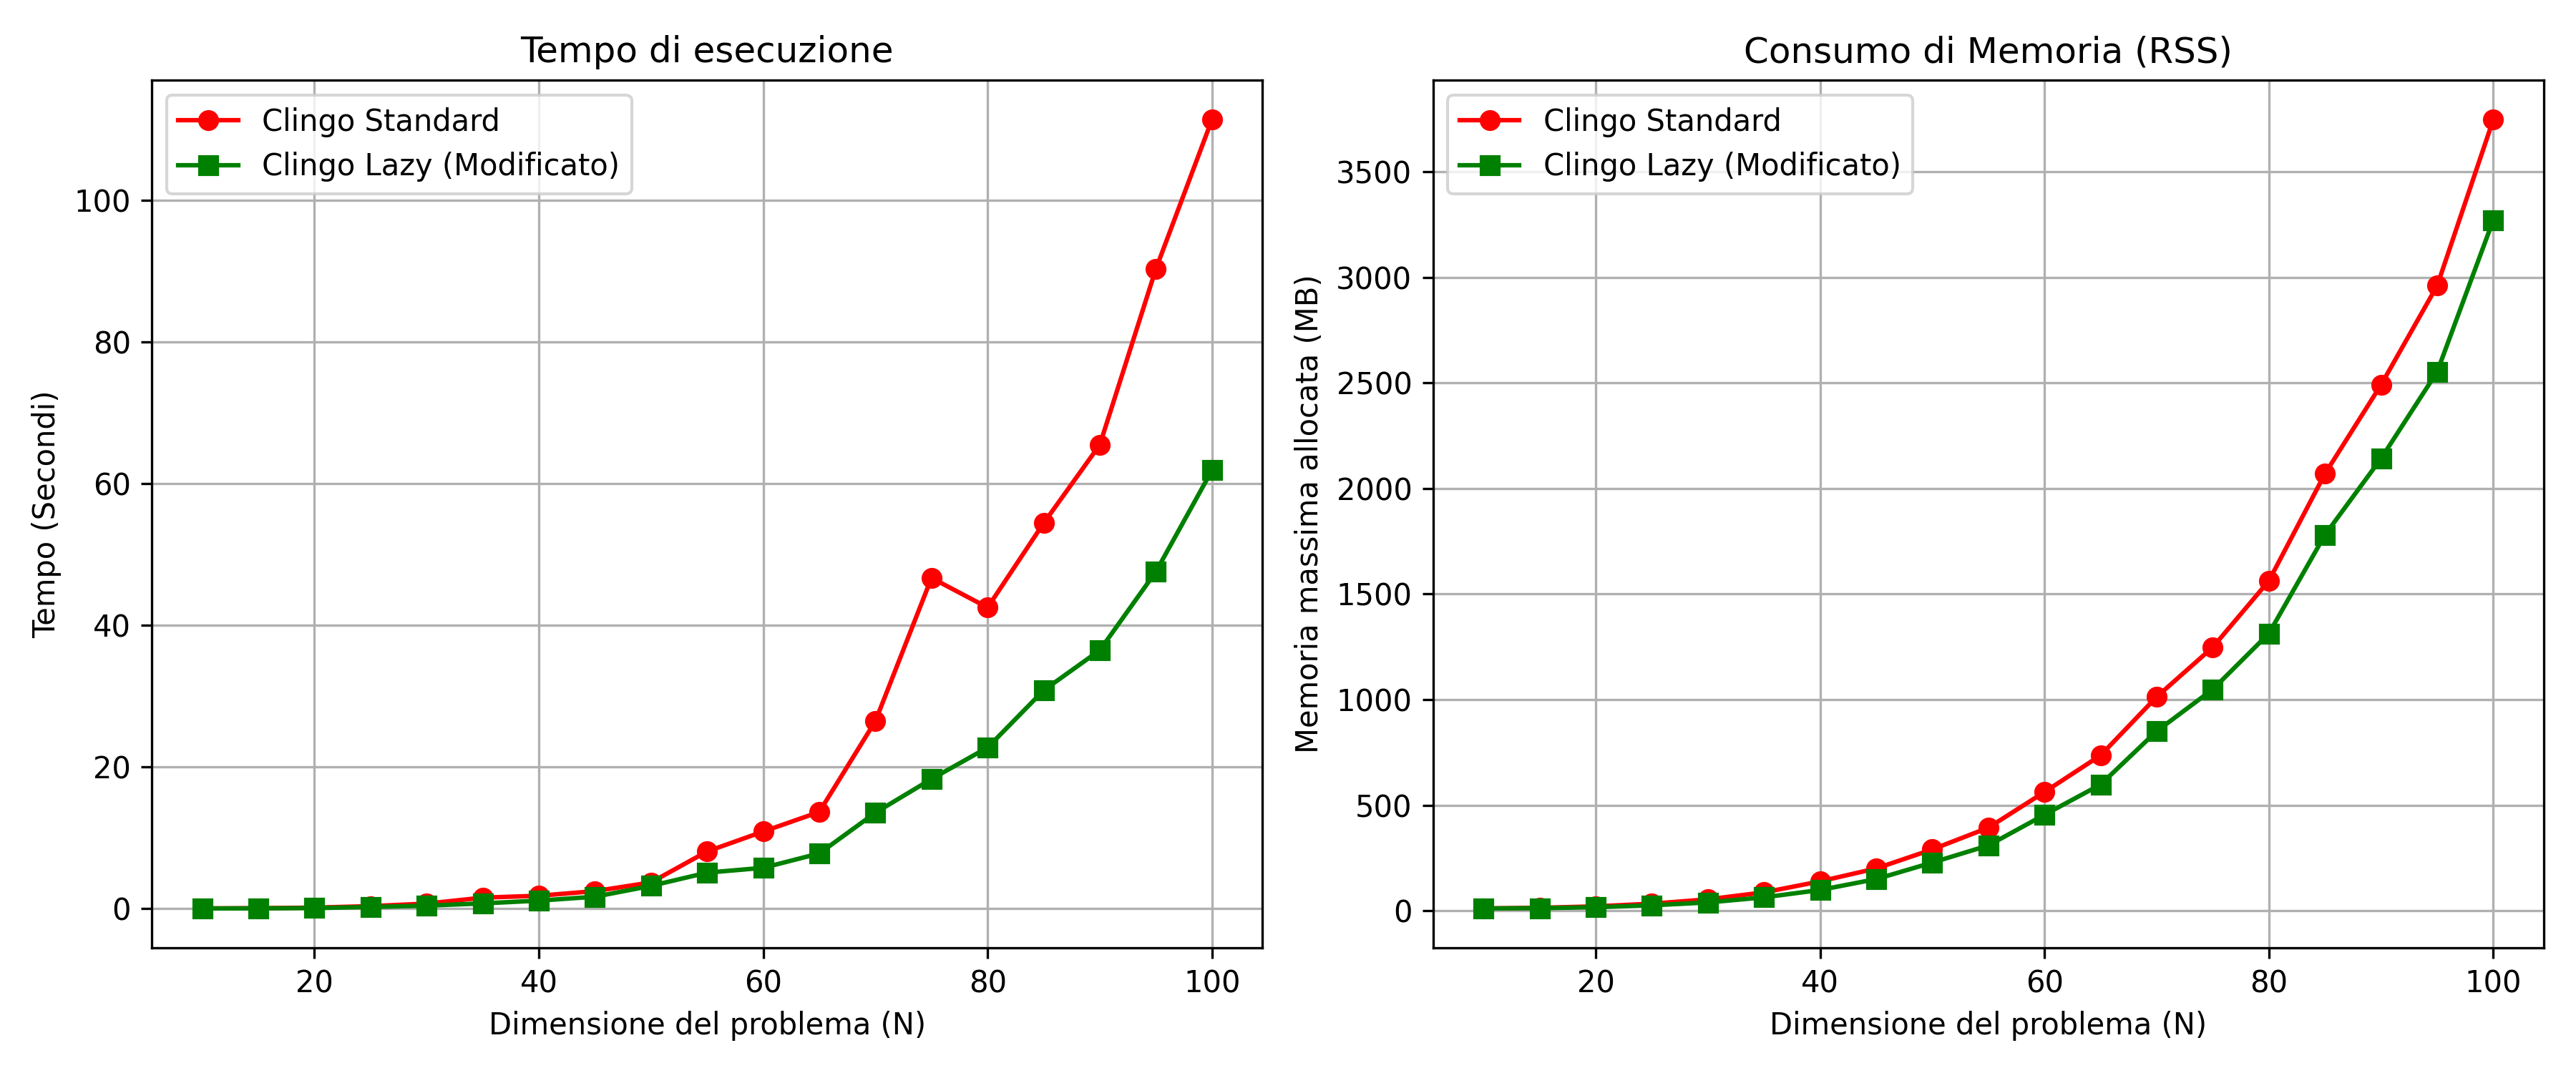
\includegraphics[width=0.9\textwidth]{../test_folder/graphs/benchmark_results.png}
    \caption{Confronto delle prestazioni: tempo di esecuzione e consumo di memoria tra Clingo Standard e Clingo con euristiche lazy (Modificato) sul Balanced Sum Problem.}
    \label{fig:benchmark_time}
\end{figure}

L'approccio con aggregati dinamici (\texttt{mod}) mostra un tempo di esecuzione significativamente inferiore rispetto alla versione standard per valori di $n$ crescenti. Questo \`{e} dovuto al fatto che:
\begin{enumerate}
    \item La fase di \emph{grounding} produce un numero lineare di regole (anzich\'{e} esponenziale).
    \item Il calcolo dell'aggregato avviene in tempo costante durante la ricerca.
    \item L'euristica \`{e} pi\`{u} accurata: il valore dell'aggregato riflette l'assegnamento parziale \emph{corrente}, non un valore pre-groundato.
\end{enumerate}

\subsection{Consumo di Memoria}

Il consumo di memoria mostra una differenza ancora pi\`{u} marcata. La versione standard deve memorizzare tutte le regole ground delle euristiche, il cui numero cresce esponenzialmente. La versione modificata mantiene solo:
\begin{itemize}
    \item $\mathcal{O}(n)$ strutture \texttt{TargetInfo} (una per direttiva euristica istanziata).
    \item $\mathcal{O}(1)$ stati aggregati (indipendenti dalla dimensione del dominio per \texttt{SumState} e \texttt{CountState}).
    \item $\mathcal{O}(n)$ watch sui letterali dei predicati aggregati.
\end{itemize}

\subsection{Analisi dei Risultati}

I risultati confermano l'ipotesi che le euristiche di dominio con aggregati dinamici migliorano notevolmente sia le prestazioni di solving che l'impronta di memoria. In particolare:

\begin{itemize}
    \item Per $n \leq 30$, entrambe le versioni terminano rapidamente, ma la versione standard inizia a mostrare un overhead significativo nella fase di grounding.
    \item Per $n \geq 50$, la versione standard diventa impraticabile a causa dell'esplosione del programma ground, mentre la versione modificata mantiene tempi di esecuzione nell'ordine delle frazioni di secondo.
    \item La curva di crescita della memoria per la versione standard mostra un andamento super-lineare (tendente all'esponenziale), mentre per la versione modificata resta essenzialmente lineare.
\end{itemize}

% ===========================================================================
% CAPITOLO 6: CONCLUSIONI E SVILUPPI FUTURI
% ===========================================================================
\chapter{Conclusioni e Sviluppi Futuri}
\label{ch:conclusioni}

\section{Riepilogo dei Contributi}

In questa tesi abbiamo presentato un'implementazione di euristiche di dominio con aggregati dinamici nel solver ASP \clingo{}, adottando un approccio basato su propagatori nativi in C++. I principali contributi sono:

\begin{enumerate}
    \item \textbf{Riscrittura delle direttive euristiche}: abbiamo proposto una trasformazione sintattica che codifica gli aggregati come funzioni non interpretate (\texttt{\_\_sum}, \texttt{\_\_count}, \texttt{\_\_min}, \texttt{\_\_max}), aggirando il grounding bottleneck.

    \item \textbf{Propagatore nativo}: abbiamo implementato il \hprop{} come estensione dell'interfaccia \texttt{Clingo::Heuristic}, integrandolo direttamente nel ciclo di ricerca del solver.

    \item \textbf{Aggregati polimorfici}: abbiamo progettato un'interfaccia \texttt{AggregateState} che consente di aggiungere nuovi tipi di aggregati senza modificare il propagatore. Le implementazioni per somma e conteggio operano in $\mathcal{O}(1)$, quelle per minimo e massimo in $\mathcal{O}(\log k)$.

    \item \textbf{Verifica della condizione}: abbiamo implementato il controllo sul letterale dell'atomo \texttt{\_\_heuristic} stesso, garantendo che le euristiche siano applicate solo quando la loro condizione \`{e} soddisfatta nell'assegnamento corrente.

    \item \textbf{Supporto per predicati n-ari}: abbiamo esteso il parser per accettare un indice opzionale dell'argomento target (\texttt{\_\_sum(pred, index)}), permettendo l'uso del propagatore su domini con predicati di arità arbitraria.

    \item \textbf{Validazione sperimentale}: i benchmark sul Balanced Sum Problem confermano che l'approccio riduce drasticamente sia il tempo di esecuzione che il consumo di memoria rispetto al grounding tradizionale delle euristiche.
\end{enumerate}

\section{Limitazioni}
\label{sec:limitazioni}

L'implementazione attuale presenta le seguenti limitazioni tecniche:

\subsection{Parser e Sintassi}

La trasformazione delle direttive euristiche nella forma \texttt{\_\_heuristic/4} \`{e} attualmente eseguita manualmente dall'utente. Un'estensione naturale sarebbe l'integrazione di un passo di pre-processing automatico (o un'estensione del parser di \clingo{}) che effettui la riscrittura trasparente:

\begin{lstlisting}
% L'utente scrive:
#heuristic b(X) : x(X), not c(X), S = #sum{Y : c(Y)}. [X@S, true]

% Il sistema genera automaticamente:
__heuristic(b(X), X, __sum(c), true) :- x(X), not c(X).
\end{lstlisting}

\subsection{Condizioni e Guardie Complesse}

Il propagatore attuale non supporta guardie sugli aggregati, ovvero espressioni nella forma:
\begin{lstlisting}
#heuristic a : #sum{Y : c(Y)} > 10. [1@1, true]
\end{lstlisting}
dove la condizione include un operatore di confronto sull'aggregato. L'estensione richiederebbe l'introduzione di un meccanismo di \emph{guard evaluation} nello stato aggregato.

\subsection{Aggregati con Espressioni Composte}

La sintassi corrente supporta solo aggregati su singoli predicati (\texttt{\_\_sum(c)}). Aggregati con tuple composte, come $\#sum\{X*Y : p(X,Y)\}$, richiederebbero un'estensione del meccanismo di estrazione del valore.

\subsection{Multi-threading}

L'implementazione attuale non \`{e} thread-safe. Gli stati aggregati sono condivisi tra tutti i thread di ricerca. Un'estensione per il solving parallelo richiederebbe stati aggregati per-thread o meccanismi di sincronizzazione.

\section{Sviluppi Futuri}

Sulla base delle limitazioni identificate, proponiamo i seguenti sviluppi futuri:

\begin{enumerate}
    \item \textbf{Riscrittura automatica}: implementazione di un modulo di pre-processing in Python (tramite l'API di \clingo{}) o in C++ (come estensione del grounder) che trasformi automaticamente le direttive \texttt{\#heuristic} con aggregati.

    \item \textbf{Guardie e operatori di confronto}: estensione dell'\texttt{AggregateState} con un metodo \texttt{evaluate(Operator op, int threshold)} per supportare condizioni complesse sugli aggregati.

    \item \textbf{Benchmark estesi}: validazione su benchmark industriali come il Partner Units Problem (PUP) e problemi di scheduling, per confermare la generalizzabilit\`{a} dell'approccio.

    \item \textbf{Integrazione con heuristic modifier}: estensione del propagatore per supportare i modificatori \texttt{sign}, \texttt{level} e \texttt{init} della direttiva \texttt{\#heuristic} di \clingo{}.

    \item \textbf{Supporto multi-thread}: implementazione di stati aggregati thread-local per il solving parallelo con portfolio.
\end{enumerate}

% ---- Bibliografia ----

\begin{thebibliography}{99}

\bibitem{gelfond1988}
M.~Gelfond and V.~Lifschitz.
\newblock The stable model semantics for logic programming.
\newblock In R.~Kowalski and K.~Bowen, editors, \emph{Proceedings of the 5th International Conference on Logic Programming}, pages 1070--1080. MIT Press, 1988.

\bibitem{gebser2012}
M.~Gebser, R.~Kaminski, B.~Kaufmann, and T.~Schaub.
\newblock \emph{Answer Set Solving in Practice}.
\newblock Synthesis Lectures on Artificial Intelligence and Machine Learning. Morgan \& Claypool, 2012.

\bibitem{gebser2019}
M.~Gebser, R.~Kaminski, B.~Kaufmann, and T.~Schaub.
\newblock Multi-shot {ASP} solving with clingo.
\newblock \emph{Theory and Practice of Logic Programming}, 19(1):27--82, 2019.

\bibitem{dodaro2016}
C.~Dodaro, P.~Gasteiger, N.~Leone, B.~Musitsch, F.~Ricca, and K.~Schekotihin.
\newblock Combining answer set programming with domain heuristics for solving hard industrial problems.
\newblock \emph{Theory and Practice of Logic Programming}, 16(5-6):653--669, 2016.

\bibitem{dodaro2019}
C.~Dodaro, M.~Alviano, W.~Faber, N.~Leone, F.~Ricca, and M.~Sirianni.
\newblock The external interface for extending {WASP}.
\newblock In \emph{Proceedings of the 35th International Conference on Logic Programming (ICLP)}, 2019.

\bibitem{dodaro2020}
C.~Dodaro, K.~Schekotihin.
\newblock Evaluating {CDCL} variable scoring schemes.
\newblock In \emph{Proceedings of the 22nd International Conference on Theory and Applications of Satisfiability Testing (SAT)}, 2020.

\bibitem{romero2021}
J.~Romero, T.~Eiter, and K.~Schekotihin.
\newblock Domain-specific heuristics in answer set programming: A declarative non-monotonic approach.
\newblock In \emph{Proceedings of the AAAI Conference on Artificial Intelligence}, 2021.

\bibitem{romero2022}
J.~Romero, T.~Eiter, and K.~Schekotihin.
\newblock Dynamic aggregates in expressive {ASP} heuristics for configuration problems.
\newblock In \emph{Proceedings of the 38th International Conference on Logic Programming (ICLP)}, 2022.

\bibitem{weinzierl2020}
A.~Weinzierl, R.~Taupe, and G.~Friedrich.
\newblock Domain-specific heuristics in lazy-grounding {ASP} solving.
\newblock In \emph{Proceedings of the 36th International Conference on Logic Programming (ICLP)}, 2020.

\bibitem{chaff2001}
M.~Moskewicz, C.~Madigan, Y.~Zhao, L.~Zhang, and S.~Malik.
\newblock Chaff: Engineering an efficient {SAT} solver.
\newblock In \emph{Proceedings of the 38th Design Automation Conference (DAC)}, pages 530--535, 2001.

\bibitem{alpha2018}
A.~Weinzierl.
\newblock Blending lazy-grounding and {CDNL} search for answer-set solving.
\newblock In \emph{Proceedings of the 14th International Conference on Logic Programming and Nonmonotonic Reasoning (LPNMR)}, pages 191--204, 2017.

\end{thebibliography}

\end{document}
